%%%%%%%%%%%%%%%%%%%%%%%%%%%%%%%%%%%%%%%%%%%%%%%%%%%%%%%%%%%%%%%%%%%%%%%%%%%%%%%%%%%%%%%%%%%%%%%%%%%


%%%%%%%%%%%%%%%%%%%%%%%%%%%%%%%%%%%%%%%%%%%%%%%%%%%%%%%%%%%%%%%%%%%%%%%%%%%%%%%%%%%%%%%%%%%%%%%%%%%
%%%%%%%%%%%%%%%%%%%%%%%%%%%%%%%%%%%%%%%%%%%%%%%%%%%%%%%%%%%%%%%%%%%%%%%%%%%%%%%%%%%%%%%%%%%%%%%%%%%
%%%%%%%%%%%%%%%%%%%%%%%%%%%%%%%%%%%%%%%%%%%%%%%%%%%%%%%%%%%%%%%%%%%%%%%%%%%%%%%%%%%%%%%%%%%%%%%%%%%

\chapter{Discusión y Conclusiones}

Considerar a las épocas, fragmentos de registros electrofisiológicos, como unidades de estudio es equivalente a considerar como unidades de estudio a las sub-capas que componen a la corteza cerebral.

-------------

Al comparar sujetos de los grupo CTRL y PDCL, no se observaron cambios estadísticamente significativos en las cantidades $\text{p}_{\text{MOR}}$ y $\text{p}_{\text{NMOR}}$, que respectivamente representan las proporciones de tiempo durante las cuales los registros de PSG se comportan como débilmente estacionario durante MOR y NMOR. 
%
En base a estos resultados, puede concluirse que los cambios en la corteza cerebral durante el PDCL no inducen cambios significativos en su \textit{comportamiento} como estacionarios;
en otras palabras, con el PDCL la actividad mantiene una parte importante de su \textit{estructura} y es false que se vuelve más \textit{simple}.
%Esto puede interpretarse como que los cambios en la corteza cerebral durante el PDCL, no provocan que  la señal se vuelva más \textit{simple} en el sentido de \textit{volverse} estacionaria.

%Este trabajo parte de la hipótesis de que adultos mayores con PDC presentan en mayor medida 
%estacionariedad débil en sus registros de PSG; al comparar sujetos de los grupo Nn (control) y Mn 
%(PDC), no se observaron cambios significativos en la porción de tiempo durante la cual el registro 
%de PSG se comporta como débilmente estacionario. 
%Esto puede interpretarse como que los cambios en la corteza cerebral durante el deterioro 
%cognitivo, no provocan que  la señal se vuelva más \textit{simple} en el sentido de 
%\textit{volverse} estacionaria.

Comparando grupalmente la cantidad de épocas estacionarias durante MOR y NMOR, se encontró que en 
el grupo CTRL había diferencias significativas en sitios de la región frontal y que no eran presentes
en el grupo PDCL; para poder establecer una relación con el PDC haría falta un mayor grupo muestral, 
o bien nuevos registros de PSG para los mismos sujetos, o incluso analizar registros de EEG durante 
otro tipo de actividades y confirmar las diferencias encontradas.

Cabe destacar que la evidencia aportada indica que el PSG es un conjunto de señales que se comportan
como no-estacionarias durante la mayor parte del sueño, lo cual confirma el supuesto usual de que 
las señales de origen biológico son por naturaleza no-estacionarias. 
%\subsection{Efecto del tamaño de las época}

%En el apéndice X se explica que si disminuye el tamaño de época el test de PSR disminuye su 
%potencia, de modo que es más propensa a dar falsos negativos (rechazar la hipótesis de 
%estacionariedad cuando debía aceptarse); entonces, en épocas más pequeñas debería haber más épocas 
%clasificadas como no-estacionarias.
%Sin embargo, al \textit{graficar} la estacionariedad para diferentes tamaños de época (figura
%\ref{comp_VCR}) ocurre que es más frecuente el efecto contrario.
%
%\begin{figure}
%\centering
%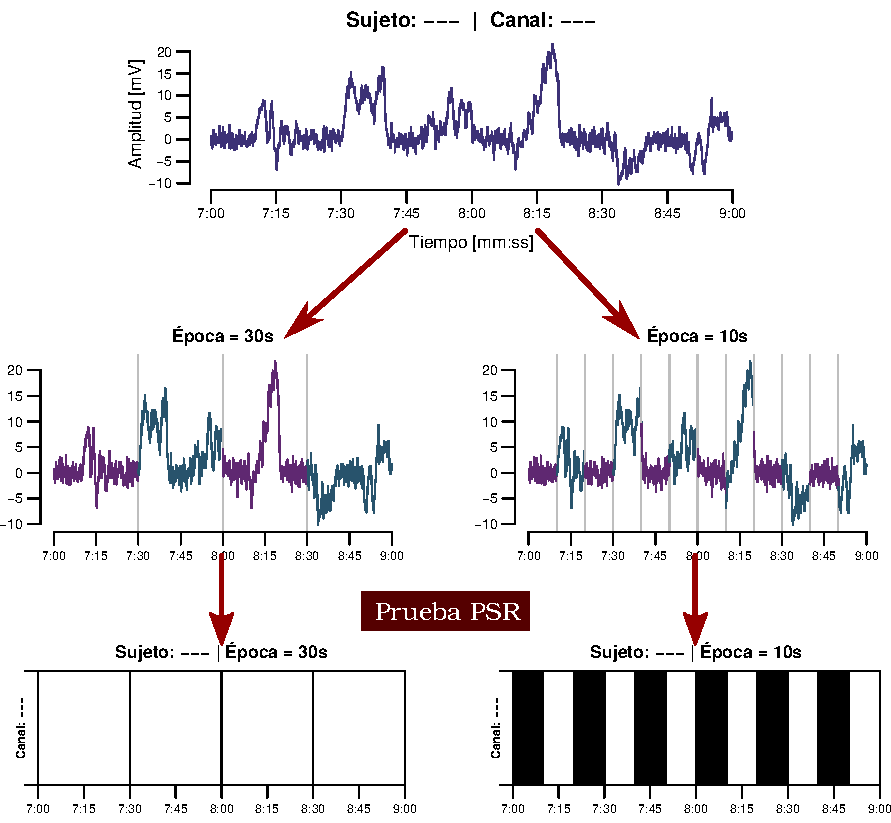
\includegraphics[width=\linewidth]{./img_diagramas/epocas_diferentes_v2.pdf}
%\caption{Efecto del tamaño de ventana sobre la clasificación de estacionariedad}
%\label{epocas_diferentes}
%\end{figure}
%
%Se propone que este efecto puede ser explicado si los registros de PSG son \textbf{localmente
%estacionarios}, una propiedad introducida por Dahlhaus \cite{Dahlhaus97} y que consiste en que un
%proceso no-estacionario pueda ser aproximado a trozos \textit{ensamblando} procesos estacionarios
%definidos para intervalos pequeños de tiempo.
%Esta caracterización del EEG ha sido usada anteriormente de manera fructífera pero problemática
%[??].
%
%En el contexto particular del presente trabajo, la presencia de estacionariedad local puede ser
%explicada fisiológicamente por el contenido heterogéneo de ritmos cerebrales de las etapas de 
%sueño; como ejemplo, en la etapa N3 aparecen husos de sueño mezcladas con ritmos Alfa, de modo
%que es posible hallar un fragmento de época en sueño N3 con únicamente un tren de ondas Alfa
%o un tren de husos de sueño.
%Este fenómeno es ilustrado de manera esquemática en la figura \ref{epocas_diferentes}.
%
%
%
%Entonces, se propone que los registros de PSG se comportan como procesos localmente estacionarios; 
%más aún, se propone que esta característica cambia cualitativamente en adultos mayores con PDC,
%para los cuales el \textit{nivel de homogeneidad} del PSG es muy similar durante MOR y NMOR.

%%%%%%%%%%%%%%%%%%%%%%%%%%%%%%%%%%%%%%%%%%%%%%%%%%%%%%%%%%%%%%%%%%%%%%%%%%%%%%%%%%%%%%%%%%%%%%%%%%%
%%%%%%%%%%%%%%%%%%%%%%%%%%%%%%%%%%%%%%%%%%%%%%%%%%%%%%%%%%%%%%%%%%%%%%%%%%%%%%%%%%%%%%%%%%%%%%%%%%%

\section{Conclusiones}

Se ha reportado que los cambios debidos al DCL están asociados con cambios en la estructura del sueño, y en particular en la etapa MOR.
%
Los resultados obtenidos indican que la clasificación de fragmentos de PSG como estacionarios responde a los cambios entre etapas de sueño, en particular al MOR.
%
Sin embargo, no se pudo establecer una relación clara entre el PDCL (una forma \textit{concreta} del DCL) y los cambios detectados usando la clasificación de estacionariedad.

Se concluye que la metodología descrita no puede usarse directamente como un marcador para el diagnóstico del PDCL.
%
Sin embargo, tampoco puede descartarse su utilidad para dicho fin, ya que muestra diferencias significativas para los patrones de actividad cerebral en regiones fisiológicamente relevantes: ??.


Respecto a la hipótesis de estacionariedad local (presentada en la sección \ref{sec:est_local}), la información recabada sugiere que dicha hipótesis se verifica para registros de PSG en adultos mayores.
%
En otras palabras, es posible que existan fragmentos arbitrariamente cortos de registros de PSG, los cuales no \textit{corresponden} a procesos estocásticos débilmente estacionarios.
%
Paralelamente, los resultados obtenidos sugieren que la presencia de dichos fragmentos se ve influida por la etapa de sueño --o quizá en general por el estado de actividad del cerebro.
%
Se hipotetiza que éste fenómeno explica los resultados {favorables} en dirección a la detección del PDCL \textit{usando} la estacionariedad; en consecuencia, un mejor entendimiento de dicho fenómeno podría usarse para mejorar la metodología respecto a la detección el PDCL.
%
%Como consecuencia directa de este fenómeno, es posible limitar los efectos \textit{distorsivos} de la no-estacionariedad, para lo cual basta un diseño experimental que distinga adecuadamente el estado de actividad a estudiar. 


%Se concluye que es posible la ocurrencia de fragmentos arbitrariamente cortos de registros de PSG que no son débilmente estacionarios. Paralelamente, la presencia de estos fragmentos se ve influida por el estado de actividad del cerebro.
%%
%Como consecuencia directa de este fenómeno, es posible limitar los efectos \textit{distorsivos} de la no-estacionariedad, para lo cual basta un diseño experimental que distinga adecuadamente el estado de actividad a estudiar. 

El hallazgo incidental de patrones emergentes de estacionariedad (ver sección \ref{sec:analisis_registro}) sugiere que, en principio, es posible usar la clasificación de estacionariedad en registros de EEG para caracterizar estados de actividad cerebral. 
%
%Para ello, falta investigar las características particulares de la etapa que se busca identificar, así como otras etapas cercanas en el tiempo.
%
Esta posibilidad es interesante, pero va más allá de los objetivos del presente trabajo.
 
%  posible usar la proporción de estacionariedad (\textit{densidad} de ventanas estacionarias en el sentido de PSR) en el EEG para caracterizar estados de actividad cerebral. Para ello, falta investigar las características particulares de la etapa que se busca identificar, así como otras etapas cercanas en el tiempo.

%%%%%%%%%%%%%%%%%%%%%%%%%%%%%%%%%%%%%%%%%%%%%%%%%%%%%%%%%%%%%%%%%%%%%%%%%%%%%%%%%%%%%%%%%%%%%%%%%%%
%%%%%%%%%%%%%%%%%%%%%%%%%%%%%%%%%%%%%%%%%%%%%%%%%%%%%%%%%%%%%%%%%%%%%%%%%%%%%%%%%%%%%%%%%%%%%%%%%%%

\section{Trabajo a futuro}

Los resultados obtenidos son \textit{prometedores}, pero no son suficientes para declarar marcadores clínicos para el PDCL basados en la metodología descrita.
%
En el contexto de la colaboración con el Laboratorio de Sueño, Emoción y Cognición, la metodología será automatizada para poder analizar el total de registros obtenidos en el estudio por Vázquez Tagle y colaboradores.
%
En base a los resultados obtenidos con un número mayor de participantes, se decidirá si se inicia un nuevo estudio para \textit{validar} la metodología descrita, o si debería descartarse.

%Una vez que se haya identificado un marcador para el PDC usando un grupo de laboratorio, conviene automatizar los análisis para su uso clínico sobre un público más general.
%
%Un uso más amplio de la técnica asegura una mayor población para poder estudiar la efectividad y sensibilidad de la prueba Y más que eso, se espera que puedan ser sinceramente beneficiosos para los pacientes. 
%
%Siguiendo el protocolo usual, los marcadores presentados no serán usados como único recurso para generar un diagnóstico clínico, sino como un apoyo a las herramientas existentes.

De manera general, el uso de marcadores basados en registros de PSG aporta una base objetivo al diagnóstico del deterioro cognitivo, y complementa los resultados más subjetivos de pruebas neuropsicológicas; esta afirmación permanece válida para una gran variedad de señales electrofisiológicas y de trastornos mentales.
%
Conviene destacar que las técnicas basadas en el EEG son relativamente poco \textit{invasivas}, de bajo costo y fácil acceso, con relación a la calidad de la información obtenida y en comparación con otras técnicas para la observación del sistema nervioso central.
%
Entonces generar marcadores diagnósticos tempranos basados en el EEG facilita su acceso para el público en general, en especial para detectar etapas tempranas del deterioro cognitivo.

En otro ámbito, los patrones emergentes de estacionariedad serán explorados en trabajos futuros.

%%%%%%%%%%%%%%%%%%%%%%%%%%%%%%%%%%%%%%%%%%%%%%%%%%%%%%%%%%%%%%%%%%%%%%%%%%%%%%%%%%%%%%%%%%%%%%%%%%%
%%%%%%%%%%%%%%%%%%%%%%%%%%%%%%%%%%%%%%%%%%%%%%%%%%%%%%%%%%%%%%%%%%%%%%%%%%%%%%%%%%%%%%%%%%%%%%%%%%%
%%%%%%%%%%%%%%%%%%%%%%%%%%%%%%%%%%%%%%%%%%%%%%%%%%%%%%%%%%%%%%%%%%%%%%%%%%%%%%%%%%%%%%%%%%%%%%%%%%%
